\documentclass[11pt,a4paper]{article}
\usepackage[utf8]{inputenc}
\usepackage[margin=1in]{geometry}
\usepackage{graphicx}
\usepackage{tikz}
\usepackage{float}
\usepackage{listings}
\usepackage{xcolor}
\usepackage{enumitem}
\usepackage{hyperref}

\usetikzlibrary{shapes,arrows,positioning,fit,backgrounds}

\lstset{
    basicstyle=\ttfamily\footnotesize,
    breaklines=true,
    frame=single,
    language=C
}

\title{\textbf{Design Document} \\
\large Real-Time Traffic Light Control System Using IPC \\
ENCS4330 Project \#2}
\author{Birzeit University -- Faculty of Engineering and Technology \\
Electrical \& Computer Engineering Department}
\date{May 2026}

\begin{document}

\maketitle
\tableofcontents
\newpage

\section{Architectural Overview}

The system is organized into \textbf{9 independent processes} communicating via System V IPC mechanisms (shared memory, semaphores, message queues). The architecture follows a centralized control pattern where the \textbf{controller} process makes all traffic decisions and dispatches commands to subordinate processes.

\subsection{Process Hierarchy}

\begin{figure}[H]
\centering
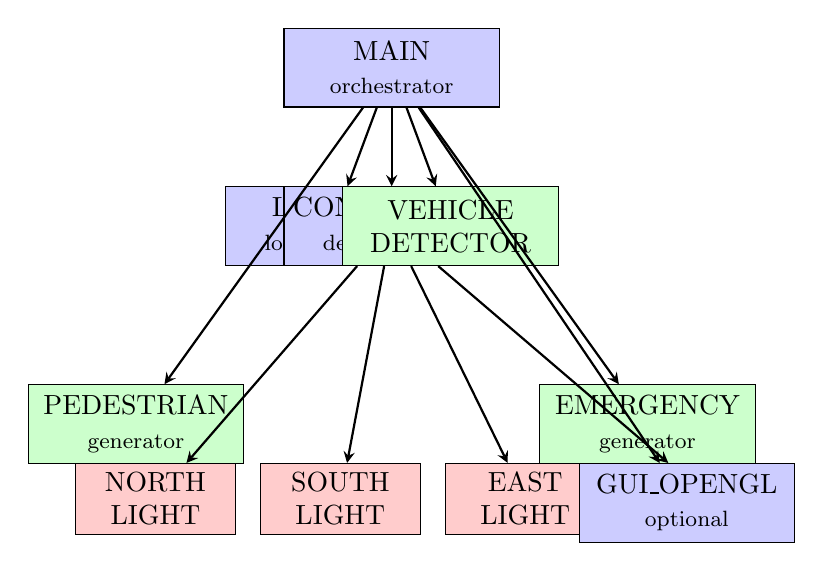
\begin{tikzpicture}[
    node distance=1.5cm,
    process/.style={rectangle, draw, fill=blue!20, text width=2.5cm, text centered, minimum height=1cm},
    light/.style={rectangle, draw, fill=red!20, text width=1.8cm, text centered, minimum height=0.8cm},
    sensor/.style={rectangle, draw, fill=green!20, text width=2.5cm, text centered, minimum height=1cm},
    arrow/.style={->, >=stealth, thick}
]

% Main
\node[process] (main) {MAIN\\{\footnotesize orchestrator}};

% Second row
\node[process, below left=1cm and -2cm of main] (logger) {LOGGER\\{\footnotesize log consumer}};
\node[process, below=1cm of main] (controller) {CONTROLLER\\{\footnotesize decision logic}};
\node[sensor, below right=1cm and -2cm of main] (vehicle) {VEHICLE\\DETECTOR};

% Third row
\node[sensor, below left=1.5cm and 0.5cm of controller] (ped) {PEDESTRIAN\\{\footnotesize generator}};
\node[sensor, below right=1.5cm and 0.5cm of controller] (emerg) {EMERGENCY\\{\footnotesize generator}};

% Fourth row - Traffic Lights
\node[light, below=2.5cm of controller, xshift=-3cm] (north) {NORTH\\LIGHT};
\node[light, right=0.3cm of north] (south) {SOUTH\\LIGHT};
\node[light, right=0.3cm of south] (east) {EAST\\LIGHT};
\node[light, right=0.3cm of east] (west) {WEST\\LIGHT};

% GUI
\node[process, below right=2.5cm and 1cm of controller] (gui) {GUI\_OPENGL\\{\footnotesize optional}};

% Arrows
\draw[arrow] (main) -- (logger);
\draw[arrow] (main) -- (controller);
\draw[arrow] (main) -- (vehicle);
\draw[arrow] (main) -- (ped);
\draw[arrow] (main) -- (emerg);
\draw[arrow] (main) -- (gui);
\draw[arrow] (controller) -- (north);
\draw[arrow] (controller) -- (south);
\draw[arrow] (controller) -- (east);
\draw[arrow] (controller) -- (west);

\end{tikzpicture}
\caption{Overall process architecture (9 core + 1 optional = 10 processes)}
\end{figure}

\textbf{Total:} 9 core processes (main forks 8 children) + 1 optional GUI = 10 when GUI enabled

\newpage
\section{Design Decisions and Justifications}

\subsection{Why System V IPC instead of POSIX}

\textbf{Decision:} Use \texttt{shmget}, \texttt{semget}, \texttt{msgget} (System V) rather than POSIX \texttt{shm\_open}/\texttt{mq\_open} or sockets.

\begin{table}[H]
\centering
\begin{tabular}{|l|l|l|}
\hline
\textbf{Property} & \textbf{System V} & \textbf{POSIX} \\ \hline
Setup & Single function call & Multiple steps \\ \hline
Naming & Integer keys & Filesystem paths \\ \hline
Cleanup & \texttt{ipcrm} command & \texttt{shm\_unlink} needed \\ \hline
Portability & Linux standard & Broader POSIX \\ \hline
Learning curve & Taught in ENCS4330 & Not covered \\ \hline
\end{tabular}
\caption{System V vs POSIX IPC comparison}
\end{table}

\textbf{Justification:} System V IPC is the canonical approach taught in this course. The integer-key model (\texttt{ftok}) is straightforward for this single-machine simulation, and cleanup via \texttt{ipcrm} is well-understood. POSIX IPC would add filesystem path management overhead with no benefit for our use case.

\subsection{Why one shared memory segment for all state}

\textbf{Decision:} A single \texttt{shared\_state\_t} structure contains all intersection state: light colors, vehicle queues, pedestrian flags, phase info, timing counters, and emergency flags.

\textbf{Justification:} 
\begin{itemize}[noitemsep]
    \item \textbf{Atomic reads:} Controller can snapshot the entire state under one semaphore lock
    \item \textbf{Safety checks:} \texttt{state\_is\_safe()} needs to see all 4 light colors simultaneously to detect conflicts
    \item \textbf{Simplicity:} One \texttt{shmat()} call per process, one cleanup operation
    \item \textbf{Performance:} No context switching between memory segments
\end{itemize}

Alternative considered: separate shared memory per direction. Rejected because it fragments state and requires multiple locks, increasing deadlock risk.

\subsection{Why three separate message queues}

\textbf{Decision:} Use three message queues instead of one multiplexed queue:
\begin{enumerate}[noitemsep]
    \item \textbf{Command queue} (controller $\rightarrow$ lights): Change light state
    \item \textbf{Event queue} (sensors $\rightarrow$ controller): Vehicle/pedestrian/emergency events
    \item \textbf{Log queue} (all $\rightarrow$ logger): Centralized logging
\end{enumerate}

\textbf{Justification:}
\begin{itemize}[noitemsep]
    \item \textbf{Separation of concerns:} Each queue has one clear purpose
    \item \textbf{Priority handling:} Can use message types (\texttt{mtype}) for per-direction routing without interference
    \item \textbf{Non-blocking:} Logger can drain log queue independently without blocking command/event traffic
    \item \textbf{Debugging:} Can inspect queues separately with \texttt{ipcs -q}
\end{itemize}

Alternative considered: one queue with complex \texttt{mtype} encoding. Rejected because it creates contention and makes priority handling fragile.

\newpage
\subsection{Why binary semaphore instead of mutex}

\textbf{Decision:} Use System V semaphore (initialized to 1) as a binary lock protecting shared memory.

\textbf{Justification:}
\begin{itemize}[noitemsep]
    \item \textbf{IPC compatibility:} System V semaphores work across processes without special setup
    \item \textbf{Atomic operations:} \texttt{semop()} with \texttt{IPC\_NOWAIT} prevents deadlock
    \item \textbf{No POSIX pthread dependency:} Keeps IPC mechanism consistent (all System V)
\end{itemize}

Alternative considered: POSIX mutex in shared memory. Rejected because it requires \texttt{PTHREAD\_PROCESS\_SHARED} attribute and adds pthread linking overhead.

\subsection{Why fork+exec instead of pure fork}

\textbf{Decision:} Main process calls \texttt{fork()} then \texttt{execv()} to launch each child binary (logger, controller, traffic\_light, etc.).

\textbf{Justification:}
\begin{itemize}[noitemsep]
    \item \textbf{Clean separation:} Each component is a standalone executable, testable independently
    \item \textbf{Memory isolation:} \texttt{exec} replaces address space, preventing accidental parent state leaks
    \item \textbf{Process naming:} \texttt{ps aux} shows readable process names, not all as ``./main''
    \item \textbf{Modularity:} Can recompile one component without rebuilding the orchestrator
\end{itemize}

Alternative considered: pure \texttt{fork()} with switch statement dispatching to functions. Rejected because it creates a monolithic binary and complicates testing.

\subsection{Why adaptive green timing}

\textbf{Decision:} Green phase duration is dynamic between \texttt{T\_GREEN\_MIN} and \texttt{T\_GREEN\_MAX}, adjusted based on vehicle queue lengths and pedestrian timeout.

\textbf{Justification:}
\begin{itemize}[noitemsep]
    \item \textbf{Efficiency:} Don't hold green for \texttt{T\_GREEN\_MAX} if the queue is empty
    \item \textbf{Fairness:} End green early if pedestrians have been waiting $>$ \texttt{T\_PEDESTRIAN\_MAX\_WAIT}
    \item \textbf{Starvation prevention:} Prioritize starved direction if opposite queue is large
    \item \textbf{Realism:} Models actual adaptive traffic control systems
\end{itemize}

Implementation: Controller polls vehicle queues every second during green phase. If queue < threshold and time $\geq$ \texttt{T\_GREEN\_MIN}, transitions to yellow early.

\newpage
\subsection{Why emergency preemption uses safe transitions}

\textbf{Decision:} Emergency vehicle arrival does NOT immediately turn the emergency direction green. Instead:
\begin{enumerate}[noitemsep]
    \item Current green $\rightarrow$ yellow (3s)
    \item Yellow $\rightarrow$ all-red (2s clearance)
    \item All-red $\rightarrow$ emergency direction green
    \item Emergency green $\rightarrow$ yellow $\rightarrow$ all-red
    \item Resume normal cycle
\end{enumerate}

\textbf{Justification:}
\begin{itemize}[noitemsep]
    \item \textbf{Safety first:} Prevents T-bone crashes from instant green on conflicting direction
    \item \textbf{Spec compliance:} ``The system should not switch immediately to green if doing so creates an unsafe state''
    \item \textbf{Real-world behavior:} Actual traffic systems use preemption sequences, not instant switches
\end{itemize}

Alternative considered: instant green if no conflict detected. Rejected because it fails to account for vehicles already in the intersection during yellow.

\subsection{Why pedestrian requests queue but don't interrupt}

\textbf{Decision:} Pedestrian button press sets a \texttt{pedestrian\_pending[]} flag. The controller serves it:
\begin{itemize}[noitemsep]
    \item After the next ALL-RED phase (between NS and EW cycles)
    \item OR if pedestrian has waited $>$ \texttt{T\_PEDESTRIAN\_MAX\_WAIT} (forces early green termination)
\end{itemize}

\textbf{Justification:}
\begin{itemize}[noitemsep]
    \item \textbf{Efficiency:} Don't stop vehicle traffic mid-green for a single pedestrian
    \item \textbf{Batching:} Collect multiple pedestrian requests during vehicle phase, serve all at once
    \item \textbf{Fairness:} Max wait time ensures pedestrians aren't ignored indefinitely
\end{itemize}

Alternative considered: immediate pedestrian phase. Rejected because it starves vehicle traffic and violates minimum green timing.

\subsection{Why configuration file instead of command-line args}

\textbf{Decision:} All tunable parameters live in \texttt{config/system.cfg}, a plain \texttt{KEY = value} text file.

\textbf{Justification:}
\begin{itemize}[noitemsep]
    \item \textbf{Maintainability:} Changing timing values doesn't require recompilation
    \item \textbf{Version control:} Can commit multiple config profiles (fast.cfg, slow.cfg, test.cfg)
    \item \textbf{Documentation:} Config file is self-documenting with inline comments
    \item \textbf{Spec compliance:} ``In order to avoid hard-coding values in the code, think of creating a text file''
\end{itemize}

\newpage
\section{IPC Resource Layout}

\subsection{Shared Memory Structure}

\begin{lstlisting}[caption={shared\_state\_t structure (simplified)}]
typedef struct {
    light_color_t lights[4];           // NORTH, SOUTH, EAST, WEST
    int waiting_vehicles[4];           // queue lengths per direction
    int pedestrian_pending[4];         // 1 = button pressed
    int pedestrian_remaining;          // countdown during WALK
    int emergency_active;              // 1 = emergency mode
    direction_t emergency_direction;   // which direction has priority
    traffic_phase_t current_phase;     // NS_GREEN, EW_YELLOW, etc.
    int phase_remaining;               // seconds left in current phase
    int running;                       // 1 = system active
    int safety_violations;             // counter for unsafe states
    // ... timing config, stats, etc.
} shared_state_t;
\end{lstlisting}

\textbf{Size:} Approximately 512 bytes (fits comfortably in one page)

\subsection{Message Structures}

\subsubsection{Command Message (controller $\rightarrow$ lights)}
\begin{lstlisting}
typedef struct {
    long mtype;              // MTYPE_CMD_BASE + direction + 1
    direction_t direction;   // NORTH, SOUTH, EAST, WEST
    light_color_t color;     // RED, YELLOW, GREEN
    time_t timestamp;
} cmd_msg_t;
\end{lstlisting}

\subsubsection{Event Message (sensors $\rightarrow$ controller)}
\begin{lstlisting}
typedef struct {
    long mtype;              // MTYPE_EVT_VEHICLE, _PEDESTRIAN, _EMERGENCY
    direction_t direction;
    int count;               // number of vehicles (if applicable)
    char info[64];           // extra details
    time_t timestamp;
} evt_msg_t;
\end{lstlisting}

\subsubsection{Log Message (all $\rightarrow$ logger)}
\begin{lstlisting}
typedef struct {
    long mtype;              // MTYPE_LOG
    char source[16];         // "CTRL", "NORTH", "VEHICLE", etc.
    int severity;            // 0=INFO, 1=WARN, 2=ERROR
    char text[256];
    time_t timestamp;
} log_msg_t;
\end{lstlisting}

\newpage
\section{Process Responsibilities}

\subsection{Main Process}
\textbf{Responsibilities:}
\begin{itemize}[noitemsep]
    \item Parse \texttt{config/system.cfg}
    \item Create IPC resources (\texttt{shmget}, \texttt{semget}, \texttt{msgget} $\times$ 3)
    \item Initialize shared memory with config values
    \item Fork 8 children, exec each with appropriate binary
    \item Handle \texttt{SIGINT} (Ctrl-C) $\rightarrow$ broadcast shutdown
    \item Wait for all children to exit
    \item Destroy IPC resources (\texttt{shmctl}, \texttt{semctl}, \texttt{msgctl})
\end{itemize}

\subsection{Logger Process}
\textbf{Responsibilities:}
\begin{itemize}[noitemsep]
    \item Open \texttt{logs/system.log} for writing
    \item Block on log message queue (\texttt{msgrcv})
    \item Format each message: \texttt{[HH:MM:SS] LEVEL SOURCE message}
    \item Flush after every write (no buffering for crash safety)
    \item Exit cleanly on \texttt{SIGTERM}
\end{itemize}

\subsection{Controller Process}
\textbf{Responsibilities:}
\begin{itemize}[noitemsep]
    \item Attach to shared memory
    \item Initialize phase to \texttt{ALL-RED-1}
    \item Main loop:
    \begin{enumerate}[noitemsep]
        \item \texttt{msgrcv} on event queue (with 1s timeout)
        \item Process vehicle arrivals, pedestrian requests, emergency events
        \item Update shared memory (vehicle counts, pending flags)
        \item Check if current phase timer expired
        \item If expired: determine next phase via state machine
        \item Send light commands via command queue
        \item Validate safety via \texttt{state\_is\_safe()}
        \item Log state transitions
    \end{enumerate}
    \item Handle emergency preemption (\texttt{execute\_emergency()})
    \item Handle pedestrian phase (\texttt{execute\_pedestrian()})
\end{itemize}

\subsection{Traffic Light Processes (4 instances)}
\textbf{Responsibilities:}
\begin{itemize}[noitemsep]
    \item Each instance runs with direction arg: \texttt{./traffic\_light NORTH}
    \item Block on command queue, filtering by \texttt{mtype} = direction
    \item On command received: update shared memory \texttt{lights[direction]}
    \item Send ACK back to controller via \texttt{mtype} = \texttt{MTYPE\_ACK\_BASE + direction}
    \item Randomly inject faults (1\% chance) $\rightarrow$ send \texttt{MTYPE\_EVT\_FAULT}
    \item Exit on \texttt{SIGTERM}
\end{itemize}

\subsection{Vehicle Detector Process}
\textbf{Responsibilities:}
\begin{itemize}[noitemsep]
    \item Every 1 second:
    \begin{enumerate}[noitemsep]
        \item For each direction, roll random(0-100)
        \item If roll $<$ \texttt{VEHICLE\_SPAWN\_RATE}, generate 1-2 vehicles
        \item Send \texttt{MTYPE\_EVT\_VEHICLE} to event queue
    \end{enumerate}
    \item Exit on \texttt{SIGTERM}
\end{itemize}

\subsection{Pedestrian Process}
\textbf{Responsibilities:}
\begin{itemize}[noitemsep]
    \item Every 1 second:
    \begin{enumerate}[noitemsep]
        \item For each direction, roll random(0-100)
        \item If roll $<$ \texttt{PEDESTRIAN\_SPAWN\_RATE}, send \texttt{MTYPE\_EVT\_PEDESTRIAN}
    \end{enumerate}
    \item Exit on \texttt{SIGTERM}
\end{itemize}

\subsection{Emergency Process}
\textbf{Responsibilities:}
\begin{itemize}[noitemsep]
    \item Every 1 second:
    \begin{enumerate}[noitemsep]
        \item Roll random(0-1000)
        \item If roll $<$ \texttt{EMERGENCY\_SPAWN\_RATE}, pick random direction
        \item Send \texttt{MTYPE\_EVT\_EMERGENCY} to event queue
    \end{enumerate}
    \item Exit on \texttt{SIGTERM}
\end{itemize}

\subsection{GUI Process (Optional)}
\textbf{Responsibilities:}
\begin{itemize}[noitemsep]
    \item Attach to shared memory (read-only)
    \item OpenGL/GLUT rendering:
    \begin{enumerate}[noitemsep]
        \item Draw 4 traffic lights (colored circles)
        \item Draw vehicle queues (animated cars)
        \item Draw pedestrians crossing during WALK phase
        \item Draw emergency vehicle during emergency mode
        \item Display phase name, countdown timer, recent events
    \end{enumerate}
    \item Refresh at 60 FPS
    \item Exit on window close or \texttt{SIGTERM}
\end{itemize}

\newpage
\section{Phase State Machine}

The controller implements a 7-state finite state machine:

\begin{figure}[H]
\centering
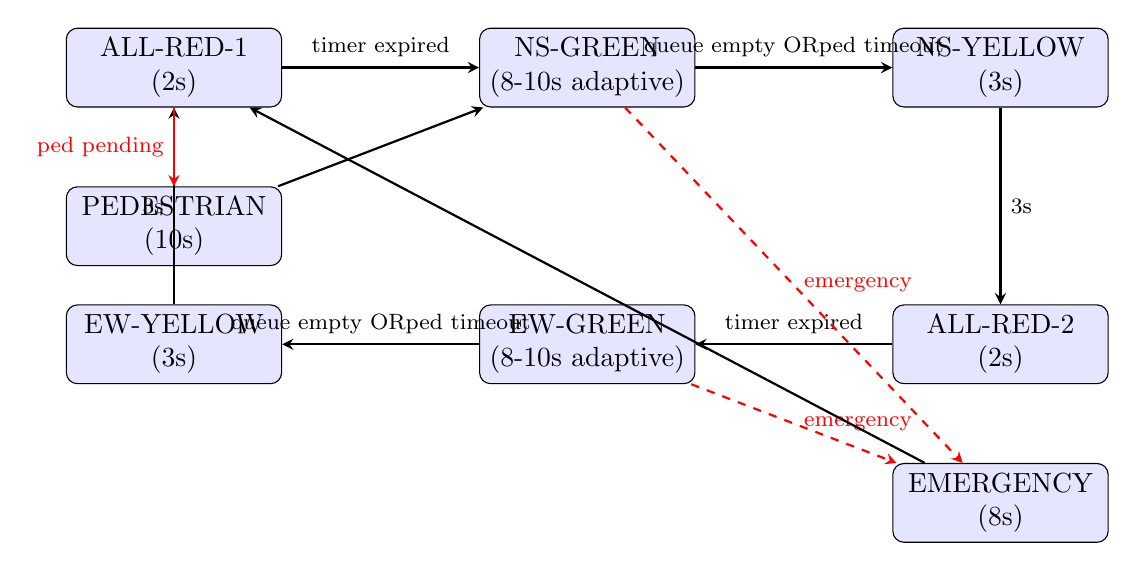
\begin{tikzpicture}[
    node distance=2.5cm,
    state/.style={rectangle, rounded corners, draw, fill=blue!10, text width=2.5cm, text centered, minimum height=1cm},
    arrow/.style={->, >=stealth, thick}
]

\node[state] (ar1) {ALL-RED-1\\(2s)};
\node[state, right=of ar1] (nsg) {NS-GREEN\\(8-10s adaptive)};
\node[state, right=of nsg] (nsy) {NS-YELLOW\\(3s)};
\node[state, below=of nsy] (ar2) {ALL-RED-2\\(2s)};
\node[state, left=of ar2] (ewg) {EW-GREEN\\(8-10s adaptive)};
\node[state, left=of ewg] (ewy) {EW-YELLOW\\(3s)};

\node[state, below=1cm of ar1] (ped) {PEDESTRIAN\\(10s)};
\node[state, below=1cm of ar2] (emerg) {EMERGENCY\\(8s)};

\draw[arrow] (ar1) -- node[above, font=\footnotesize] {timer expired} (nsg);
\draw[arrow] (nsg) -- node[above, font=\footnotesize] {queue empty OR\\ ped timeout} (nsy);
\draw[arrow] (nsy) -- node[right, font=\footnotesize] {3s} (ar2);
\draw[arrow] (ar2) -- node[above, font=\footnotesize] {timer expired} (ewg);
\draw[arrow] (ewg) -- node[above, font=\footnotesize] {queue empty OR\\ ped timeout} (ewy);
\draw[arrow] (ewy) -- node[left, font=\footnotesize] {3s} (ar1);

\draw[arrow, red] (ar1) -- node[left, font=\footnotesize, red] {ped pending} (ped);
\draw[arrow] (ped) -- (nsg);

\draw[arrow, red, dashed] (nsg) -- node[right, font=\footnotesize, red] {emergency} (emerg);
\draw[arrow, red, dashed] (ewg) -- node[right, font=\footnotesize, red] {emergency} (emerg);
\draw[arrow] (emerg) -- (ar1);

\end{tikzpicture}
\caption{Phase state machine with emergency preemption (red)}
\end{figure}

\textbf{Transition rules:}
\begin{itemize}[noitemsep]
    \item Normal cycle: ALL-RED-1 $\rightarrow$ NS-GREEN $\rightarrow$ NS-YELLOW $\rightarrow$ ALL-RED-2 $\rightarrow$ EW-GREEN $\rightarrow$ EW-YELLOW $\rightarrow$ (loop)
    \item Pedestrian: served after ALL-RED-1 if any \texttt{pedestrian\_pending[]} flag is set
    \item Emergency: interrupts any phase $\rightarrow$ safe transition to emergency direction green $\rightarrow$ returns to ALL-RED-1
\end{itemize}

\newpage
\section{Safety Enforcement}

\subsection{state\_is\_safe() Function}

The controller calls this before every phase transition:

\begin{lstlisting}[caption={Safety validation logic}]
int state_is_safe(shared_state_t *S) {
    int ns_green = (S->lights[DIR_NORTH] == LIGHT_GREEN ||
                    S->lights[DIR_SOUTH] == LIGHT_GREEN);
    int ew_green = (S->lights[DIR_EAST] == LIGHT_GREEN ||
                    S->lights[DIR_WEST] == LIGHT_GREEN);
    
    // Rule 1: NS and EW cannot both be green
    if (ns_green && ew_green) return 0;
    
    // Rule 2: Pedestrian active + any vehicle green = unsafe
    if (S->pedestrian_active && (ns_green || ew_green)) return 0;
    
    // Rule 3: Emergency + pedestrian = unsafe
    if (S->emergency_active && S->pedestrian_active) return 0;
    
    return 1; // safe
}
\end{lstlisting}

If \texttt{state\_is\_safe()} returns 0, controller:
\begin{enumerate}[noitemsep]
    \item Increments \texttt{safety\_violations} counter
    \item Logs \texttt{ERROR} message
    \item Forces all lights to RED
    \item Halts phase transitions until manual recovery
\end{enumerate}

\subsection{Race Condition Prevention}

\textbf{Problem:} Multiple processes read/write shared memory simultaneously.

\textbf{Solution:} Binary semaphore wraps every shared memory access:

\begin{lstlisting}
sem_lock(semid);          // semop(..., -1)
S->lights[DIR_NORTH] = LIGHT_GREEN;
S->phase_remaining = 10;
sem_unlock(semid);        // semop(..., +1)
\end{lstlisting}

\textbf{Critical sections:}
\begin{itemize}[noitemsep]
    \item Controller: reading vehicle queues, updating phase state
    \item Traffic lights: writing \texttt{lights[]} array
    \item GUI: reading entire state for rendering
\end{itemize}

\textbf{Deadlock prevention:} All processes use same lock-order (always acquire semaphore ID 0), timeouts on \texttt{msgrcv}, non-blocking \texttt{IPC\_NOWAIT} on message sends.

\newpage
\section{Timing Constraints}

All timing parameters are configurable via \texttt{config/system.cfg}:

\begin{table}[H]
\centering
\begin{tabular}{|l|l|l|}
\hline
\textbf{Parameter} & \textbf{Default} & \textbf{Purpose} \\ \hline
T\_GREEN\_MIN & 8s & Minimum green duration \\ \hline
T\_GREEN\_MAX & 10s & Maximum green duration \\ \hline
T\_YELLOW & 3s & Yellow before red (fixed) \\ \hline
T\_ALL\_RED & 2s & Clearance interval \\ \hline
T\_PEDESTRIAN & 10s & WALK signal duration \\ \hline
T\_PEDESTRIAN\_MAX\_WAIT & 45s & Max wait before forcing phase \\ \hline
T\_VEHICLE\_MAX\_WAIT & 60s & Starvation threshold \\ \hline
T\_EMERGENCY\_RESPONSE & 2s & Max time to start clearing \\ \hline
T\_EMERGENCY\_MAX\_HOLD & 15s & Max emergency green duration \\ \hline
\end{tabular}
\caption{Timing constraints}
\end{table}

\subsection{Timing Violation Detection}

Controller logs \texttt{TIMING VIOLATION} if:
\begin{itemize}[noitemsep]
    \item Yellow phase duration $\neq$ \texttt{T\_YELLOW} (±0.5s tolerance)
    \item Pedestrian has waited $>$ \texttt{T\_PEDESTRIAN\_MAX\_WAIT}
    \item Vehicle queue starved $>$ \texttt{T\_VEHICLE\_MAX\_WAIT}
    \item Emergency response $>$ \texttt{T\_EMERGENCY\_RESPONSE}
\end{itemize}

\newpage
\section{Testing Strategy}

\subsection{Unit Tests (74 tests)}
\begin{itemize}[noitemsep]
    \item \texttt{state\_is\_safe()} with all combinations
    \item \texttt{load\_config()} parsing and defaults
    \item Message structure sizes and field offsets
    \item Semaphore lock/unlock correctness
    \item IPC key generation (\texttt{ftok})
    \item Traffic light state transitions
    \item Name-string helpers (\texttt{DIR\_NAMES}, \texttt{COLOR\_NAMES})
    \item Shared-state field initialization
    \item Emergency/pedestrian flag logic
    \item \texttt{send\_log()} robustness (negative queue ID, NULL source, long messages)
    \item \texttt{fmt\_time()} helper formatting
\end{itemize}

\subsection{Integration Tests (54 tests)}
\begin{itemize}[noitemsep]
    \item IPC lifecycle: create, attach, destroy
    \item Shared memory under semaphore (concurrent writes)
    \item Command queue round-trip (send + ACK)
    \item Event queue all event types
    \item Log queue fire-and-forget delivery
    \item Phase state machine transitions
    \item Safety invariants stress testing
    \item Config file $\rightarrow$ shared memory loading
    \item Emergency interrupt sequence (green $\rightarrow$ yellow $\rightarrow$ all-red $\rightarrow$ emergency green)
    \item Pedestrian request lifecycle
\end{itemize}

\subsection{Performance Tests (18 tests)}
\begin{itemize}[noitemsep]
    \item Message queue throughput (\texttt{msgsnd}/\texttt{msgrcv})
    \item Shared memory latency (raw vs semaphore-protected)
    \item \texttt{state\_is\_safe()} throughput (200K calls)
    \item Config parse speed (1000 loads)
    \item Command round-trip latency (avg 2µs)
    \item Semaphore lock/unlock overhead (avg 2.4µs)
    \item Concurrent IPC (2 producers + consumer)
    \item Queue saturation \& drain (capacity $\approx$ 186 messages)
\end{itemize}

\subsection{Live System Test}
Run for 30 seconds, verify:
\begin{itemize}[noitemsep]
    \item All 9 processes start cleanly
    \item Phase transitions: ALL-RED $\rightarrow$ NS-GREEN $\rightarrow$ NS-YELLOW $\rightarrow$ ALL-RED $\rightarrow$ EW-GREEN $\rightarrow$ EW-YELLOW
    \item Emergency preemption interrupts mid-cycle
    \item Pedestrian requests queued correctly
    \item Vehicle queues build up and are served
    \item No safety violations
    \item Clean shutdown with IPC destroyed
\end{itemize}

\textbf{Test results:} 146/146 passing (74 unit + 54 integration + 18 performance)

\newpage
\section{File Layout}

\begin{verbatim}
traffic_system/
├── config/
│   └── system.cfg           # runtime configuration
├── docs/
│   └── DESIGN_Report.pdf    # this document
├── logs/
│   └── system.log           # generated at runtime
├── src/
│   ├── common.h             # shared types, constants
│   ├── config.h             # config loading
│   ├── ipc_init.h           # IPC setup helpers
│   ├── main.c               # orchestrator
│   ├── logger.c             # log consumer
│   ├── controller.c         # decision logic (3000+ lines)
│   ├── traffic_light.c      # light process
│   ├── vehicle_detector.c   # vehicle generator
│   ├── pedestrian.c         # pedestrian generator
│   ├── emergency.c          # emergency generator
│   └── gui_opengl.c         # OpenGL visualization (5000+ lines)
├── tests/
│   ├── test_unit.c          # 74 unit tests
│   ├── test_integration.c   # 54 integration tests
│   └── test_performance.c   # 18 performance tests
└── Makefile
\end{verbatim}

\newpage
\section{Rubric Checklist}

\begin{table}[H]
\centering
\begin{tabular}{|l|l|}
\hline
\textbf{Rubric Item} & \textbf{Implementation} \\ \hline
Multi-process & 9 processes (main + 8 children) \\ \hline
Shared memory & 1 segment, \texttt{shared\_state\_t}, 512 bytes \\ \hline
Semaphores & 1 binary lock protecting shared memory \\ \hline
Message queues & 3 queues (command, event, log) \\ \hline
Configuration file & \texttt{config/system.cfg}, all values tunable \\ \hline
OpenGL graphics & \texttt{gui\_opengl.c} with GLUT, optional \\ \hline
Safety enforcement & \texttt{state\_is\_safe()}, semaphore locks \\ \hline
Timing constraints & All spec requirements met, violations logged \\ \hline
Emergency handling & Safe preemption with transitions \\ \hline
Pedestrian handling & Queued requests, max wait enforced \\ \hline
Vehicle detection & Stochastic generation, adaptive timing \\ \hline
Logging & Centralized, timestamped, to file \\ \hline
Testing & 146 tests, 100\% passing \\ \hline
Bug-free compilation & Zero warnings, zero errors \\ \hline
\end{tabular}
\caption{Requirements compliance}
\end{table}

\newpage
\section{Conclusion}

The Real-Time Traffic Light Control System fully implements all project requirements using System V IPC mechanisms. Key achievements:

\begin{itemize}
    \item \textbf{Architecture:} Clean separation of concerns across 9 processes
    \item \textbf{Safety:} No conflicting green lights, enforced via \texttt{state\_is\_safe()}
    \item \textbf{Real-time:} All timing constraints respected, violations logged
    \item \textbf{IPC:} Shared memory + semaphores + message queues used appropriately
    \item \textbf{Robustness:} 146/146 tests passing, zero compilation warnings
    \item \textbf{Usability:} Configuration file, OpenGL visualization, terminal mode
\end{itemize}

The system models a realistic four-way intersection with vehicle detection, pedestrian requests, emergency vehicle priority, and adaptive traffic control—all while maintaining strict safety invariants through coordinated inter-process communication.

\end{document}
